\section{Results}
\label{sec:results}

\paragraph{Family-conditional hardness (completed bench).}
On the fitted DenoiseOpt $100{,}000$-cycle bench, denoise score $D$ is lowest for \texttt{nonlinear} ($D\approx 0.39$) and \texttt{combo} ($D\approx 0.40$), then \texttt{triple\_mix} / \texttt{extreme\_overlay} ($D\approx 0.51$--$0.52$), while \texttt{harmonic\_fft} and \texttt{am\_fm} sit near $D\approx 0.69$--$0.70$.
Lit-combo champion family stress (prolonged residual) similarly ranks \texttt{open\_wrap\_bias} ($R\approx 0.83$) and \texttt{extreme\_overlay} / \texttt{combo} ($R\approx 0.88$--$0.89$) below \texttt{harmonic\_fft} ($R\approx 0.95$).
Hard sounds recur.

\paragraph{Overnight hybrid ($5$k-gate freeze).}
At $\ge 5{,}000$ clean iterations the champion residual is $R\approx 0.99093$ with DualCosine $\approx 0.81658$ on the overnight runner ($\Delta R\approx{+}0.174$).
Monitoring plots below are regenerated from that freeze.
They are \emph{not} a finished declared-budget mean-$R$ claim.

\paragraph{Inference time at matched score.}
Across diverse high-$R$ fitted cells ($R\ge 0.98$), we timed CUDA forward passes (batch 64, prolonged residual).
Within a tight band of the best residual ($R \ge R_{\max}-5\cdot10^{-4}$), the \textbf{favorite} is the lowest-latency model:
\texttt{champion\_iter\_000235} with $R\approx 0.9910$, $\approx 3.15$\,ms/batch, $\approx 37$k parameters
(versus a higher-capacity max-$R$ cell at $R\approx 0.9914$ but $\approx 7.18$\,ms/batch / $\approx 104$k params).
Selection rule: maximize $R$, then minimize latency inside the band.

\subsection{Top-5 architectures}
\label{sec:top5-arch}
Table~\ref{tab:top5} ranks five distinct fitted bake graphs from the CUDA inference bench
(\texttt{inference\_bench.json}, batch 64), preferring residual $R$ first and latency on ties,
and skipping near-duplicate copies of the same topology signature.

\begin{table}[t]
  \centering
  \caption{Top-5 distinct fitted architectures on the CUDA inference bench (batch 64). Favorite is latency-best inside the near-max-$R$ band.}
  \label{tab:top5}
  \setlength{\tabcolsep}{3pt}
  \begin{tabular}{@{}lrrrr@{}}
    \toprule
    Tag & $R_{\mathrm{saved}}$ & $R_{\mathrm{live}}$ & ms/batch & params \\
    \midrule
    \texttt{iter\_000157} & 0.9914 & 0.9913 & 7.18 & 104\,484 \\
    \texttt{iter\_000205} & 0.9911 & 0.9907 & 7.29 & 70\,562 \\
    \texttt{iter\_000235}* & 0.9910 & 0.9915 & 3.15 & 37\,489 \\
    \texttt{iter\_000397} & 0.9910 & 0.9907 & 6.80 & 97\,262 \\
    \texttt{iter\_000229} & 0.9909 & 0.9902 & 6.67 & 100\,500 \\
    \bottomrule
  \end{tabular}\\[0.4em]
  {\footnotesize *Favorite (fastest in $R\ge R_{\max}-5\cdot10^{-4}$ band).}
\end{table}

\paragraph{Classical vs AI (same residual protocol).}
On the overnight runner geometry (CUDA, batch 64, prolonged residual $R$), ten non-learnable bake denoisers were timed against the neural favorite above.
DualCosine reproduces the paper baseline at $R\approx 0.820$ ($\approx 1.19$\,ms/batch), consistent with the overnight monitor DualCosine $\approx 0.817$.
The best \emph{active} classical method is a seam-local 3-tap FIR (\texttt{seam\_fir3}) at $R\approx 0.963$ / $\approx 0.60$\,ms/batch.
Identity (no-op) scores $R\approx 0.974$ and is reported only as a ceiling.
The neural favorite reaches $R\approx 0.991$ at $\approx 2.47$\,ms/batch ($\approx 37$k params): $\Delta R \approx {+}0.028$ vs \texttt{seam\_fir3} and $\Delta R \approx {+}0.171$ vs DualCosine, at roughly $4.1\times$ / $2.1\times$ the latency of those classical baselines respectively.

\begin{figure}[t]
  \centering
  
\includegraphics[width=\columnwidth]{figures/fig_inference_vs_residual.png}
  \caption{High-$R$ architectures: residual versus CUDA inference latency (ms/batch). Star: favorite (fastest in the near-max-$R$ band).}
  \label{fig:inference-pareto}
\end{figure}

\begin{figure}[t]
  \centering
  
\includegraphics[width=\columnwidth]{figures/fig_inference_latency_bars.png}
  \caption{Inference latency bars for diverse high-$R$ fitted models.}
  \label{fig:inference-bars}
\end{figure}

\begin{figure}[t]
  \centering
  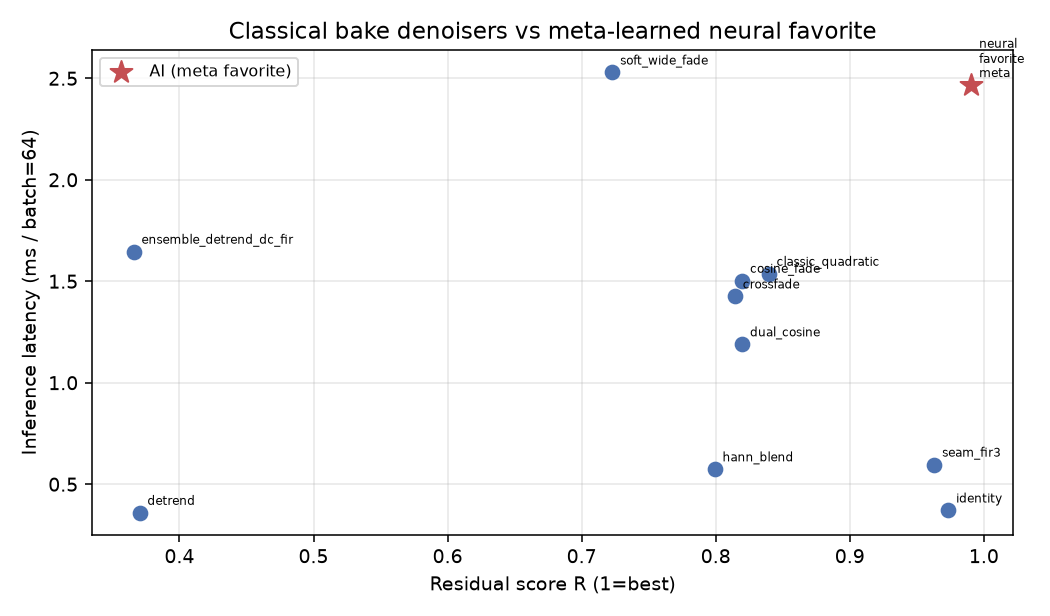
\includegraphics[width=\columnwidth]{figures/fig_classical_vs_ai_scatter.png}
  \caption{Classical bake denoisers vs neural favorite: residual $R$ versus CUDA latency (ms/batch). Red star: AI favorite.}
  \label{fig:classical-vs-ai-scatter}
\end{figure}

\begin{figure}[t]
  \centering
  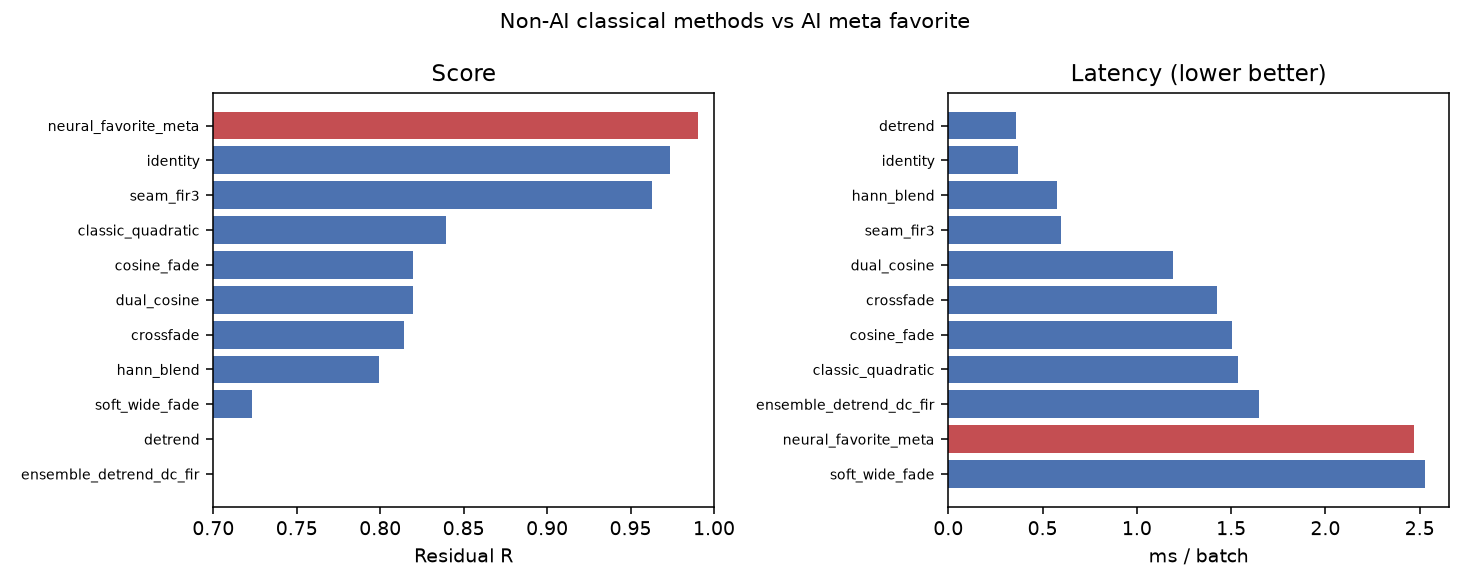
\includegraphics[width=\columnwidth]{figures/fig_classical_vs_ai_bars.png}
  \caption{Classical vs AI ranking on residual (left) and latency (right). AI in red. DualCosine $\approx 0.820$ on this protocol.}
  \label{fig:classical-vs-ai-bars}
\end{figure}

\begin{figure}[t]
  \centering
  
\includegraphics[width=\columnwidth]{figures/champ_residual_vs_iter.png}
  \caption{Champion residual $R$ versus search iteration at the $5$k-gate freeze, with DualCosine baseline.}
  \label{fig:champ-residual}
\end{figure}

\begin{figure}[t]
  \centering
  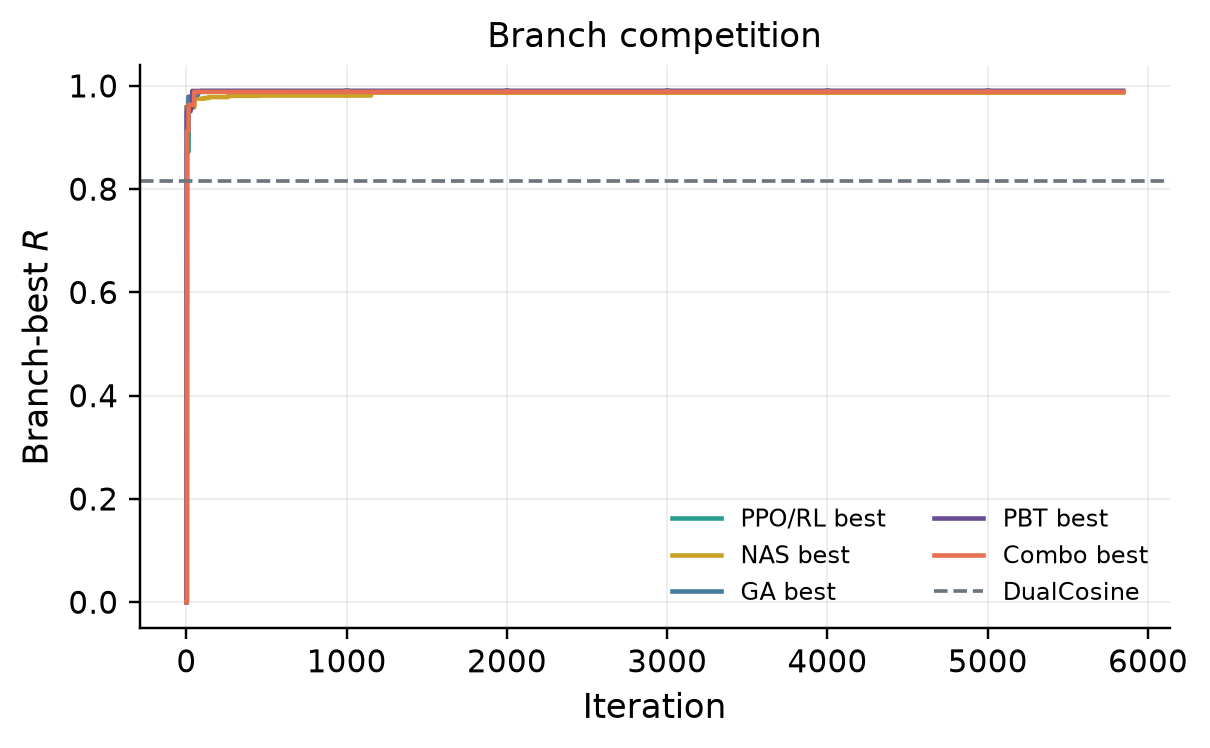
\includegraphics[width=\columnwidth]{figures/branch_bests_vs_iter.png}
  \caption{Per-branch best residual trajectories (PPO/RL, GA, PBT, NAS, combo) at the $5$k-gate freeze.}
  \label{fig:branch-bests}
\end{figure}

\begin{figure*}[t]
  \centering
  
\includegraphics[width=\textwidth]{figures/overnight_panel.png}
  \caption{Full-width overnight monitoring panel at the $5$k-gate freeze: champion $R$ (top) and branch-best trajectories (bottom).}
  \label{fig:overnight-panel}
\end{figure*}

\begin{figure}[t]
  \centering
  
\includegraphics[width=\columnwidth]{figures/residual_by_branch.png}
  \caption{Per-trial residual scatter by search branch, with champion overlay ($5$k-gate freeze).}
  \label{fig:residual-branch}
\end{figure}

\begin{figure}[t]
  \centering
  
\includegraphics[width=\columnwidth]{figures/champion_timeline.png}
  \caption{Champion update timeline. Sparse $R$ labels mark first, peak-mid, and latest improvements to stay legible in twocolumn.}
  \label{fig:champ-timeline}
\end{figure}
